\chapter{Materiais e Métodos}
\label{Materiais}

%\textcolor{red}{\textbf{Dica:} Materiais e Métodos: descrição clara dos procedimentos e dos materiais
%adotados para o desenvolvimento do trabalho (sem resultados) ? incluindo sua
%adequação ao trabalho.
%Tem que responder às perguntas:
%-está com um tamanho adequado (proporcional) à monografia?
%-há informação suficiente e clara sobre os materiais e sobre os métodos
%adotados?
%Não há necessidade de reproduzir (copiar) as obras que embasam o trabalho e
%sim colocar o suficiente para o entendimento do trabalho e citar as referências.}

Nesta seção serão apresentados os equipamentos necessários e métodos utilizados para o desenvolvimento do projeto. No caso dos equipamentos, serão apresentados todas as especificações técnicas e sua importância para o trabalho. Na seção destinada aos métodos, os algoritmos desenvolvidos para identificação e reconhecimento de objetos serão descritos.

%------------------------------------ Materiais -----------------------------------------------------
\section{Materiais}
Com relação aos equipamentos é possível classificá-los em três grupos distintos:
Câmeras estereoscópicas, Unidades de Processamento, e Equipamentos auxiliares.

\subsection{Câmeras estereoscópicas}

O projeto já utilizou duas câmeras estereoscópicas. Primeiramente, utilizou-se a \textit{webcam} Minoru(veja figura \ref{minoru}), visto que apresentava preço totalmente acessível e cumpria o requisito de realizar \textit{streaming} via USB. Deste modo, tornou-se um equipamento essencial para a implementação dos métodos para encontro de correspondências entre as câmeras. A tabela \ref{minoru_tab}	 apresenta as especificações da \textit{webcam}.

\begin{figure}[H]
 	\centering
 	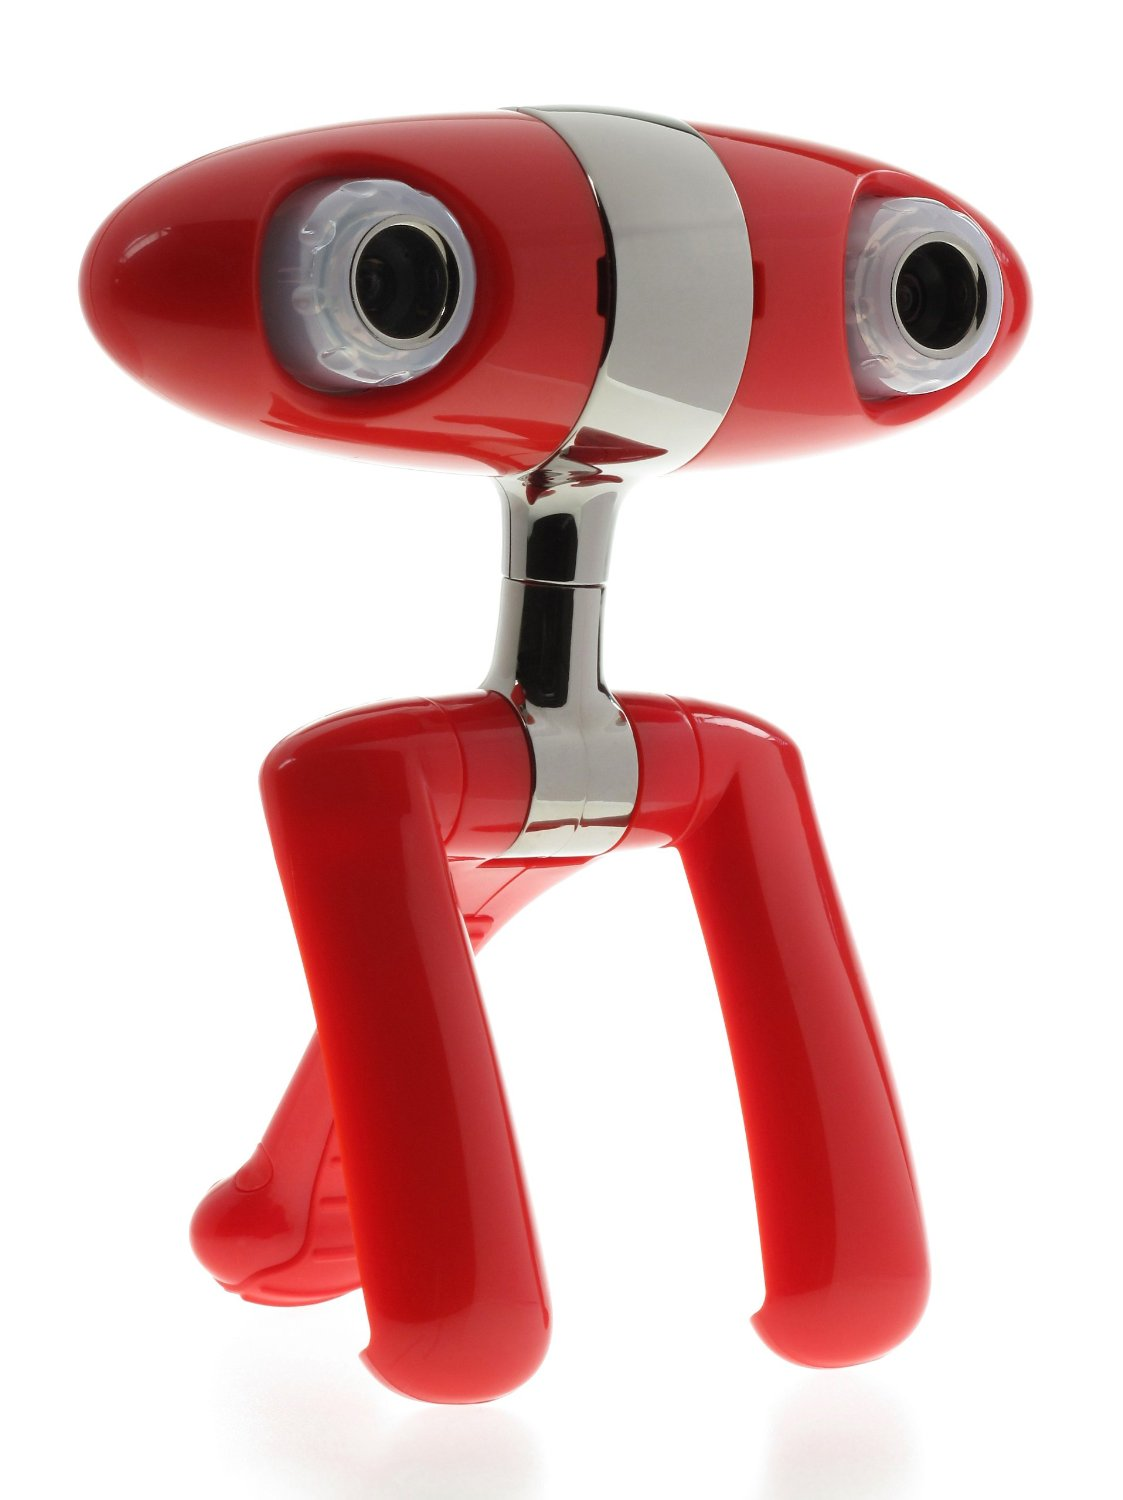
\includegraphics[scale=0.10]{./Resources/minoru.jpg}
 	\caption{3D Webcam Minoru}
 	\label{minoru}
\end{figure}

\begin{table}[]
\centering
\caption{Especificações - 3D Webcam Minoru}
\label{minoru_tab}
\begin{tabular}{ll}
\textbf{Sensor de Imagem}      & VGA CMOS Sensor  	\\
\textbf{Resolução Máxima}      & $800x600$        	\\
\textbf{Tamanho Linha de Base} & 6 cm             	\\
\textbf{Taxa de Captura}       & 30 fps             	\\
\textbf{Distância Focal}       & 10 cm até $\infty$	\\
\textbf{Campo de Visão}        & $42\degree$		   	\\
\textbf{Peso}				  & 249.48 g				\\
\end{tabular}
\end{table}

Atualmente, a câmera utilizada é uma câmera digital 3D W3 fabricada pela Fujifilm (veja figura \ref{fujiW3}). A primeira câmera foi substituída, pois o controlador USB não permitia que a webcam realizasse \textit{streaming} na máxima resolução. Deste modo, optou-se por uma câmera com maior resolução e que apresentasse lentes com baixa distorção. Entretanto, essa câmera não apresenta \textit{streaming} via USB, assim é necessário que os vídeos sejam processados \textit{offline}. Visto que o projeto preocupa-se principalmente na identificação de obstáculos, isso não oferece nenhuma desvantagem para o desenvolvimento do algoritmo. Todavia, para uma aplicação real, a câmera instalada no veículo deve apresentar esse aspecto. A tabela \ref{fujiW3_tab} apresenta as especificações da câmera.

\begin{table}[]
\centering
\caption{Especificações - Câmera Digital Fujifilm FinePix Real 3D W3}
\label{fujiW3_tab}
\begin{tabular}{ll}
\textbf{Sensor de Imagem}      & 10 MP CCD Sensor  	\\
\textbf{Resolução Máxima}      & $1280x720$        	\\
\textbf{Tamanho Linha de Base} & 7.5 cm             	\\
\textbf{Taxa de Captura}      & 24 - 30 fps          \\
\textbf{Distância Focal}       & 60 cm até $\infty$	\\
\textbf{Peso}       		      & 250g					\\
\end{tabular}
\end{table}

\begin{figure}[H]
 	\centering
 	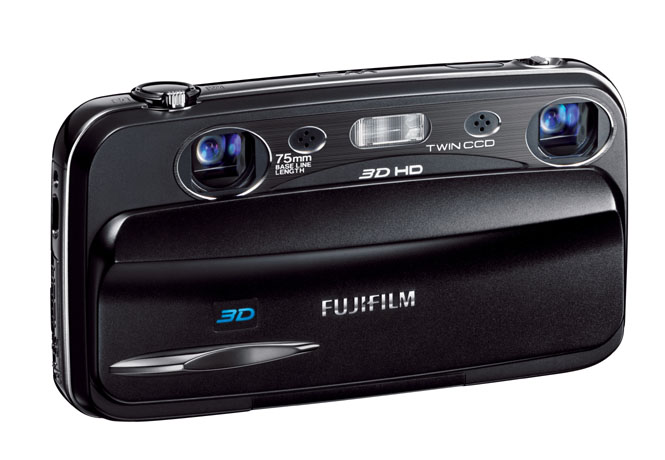
\includegraphics[scale=0.35]{./Resources/fujiW3.jpg}
 	\caption{Câmera Digital Fujifilm FinePix Real 3D W3}
 	\label{fujiW3}
\end{figure}

\subsection{Unidades de Processamento}

Visto que este trabalho também busca a implementação dos algoritmos de detecção de obstáculos em quadricópteros, tem-se como objetivo sua implementação para Linux embarcado. Abaixo estão apresentadas as plataformas que serão utilizadas para este propósito.

A primeira plataforma a ser utilizada e estudada é a plataforma aberta BeagleBone Black, ilustrada na figura \ref{bbb}. Esta plataforma foi escolhida devido ao seu tamanho reduzido, podendo ser facilmente embarcado, e ao seu poder de processamento, utiliza Cortex-A8 operando à 1 GHz. A tabela \ref{bbb_tab} apresenta as especificações da plataforma.

\begin{table}[]
\centering
\caption{Especificações - BeagleBone Black}
\label{bbb_tab}
\begin{tabular}{ll}
\textbf{Processador}           & 1GHz TI Sitara AM3359 ARM Cortex-A8					 \\
\textbf{RAM}                   & 512 MB DDR3L @ 400 MHz								 \\
\textbf{Armanezamento}         & 2 GB on-board eMMC, MicroSD                   		 \\
\textbf{Sistemas Operacionais} & Angstrom (Default), Ubuntu, Android, dentre outros...	 \\
\textbf{Consumo de energia}    & 210-460 mA @ 5V                                      	 \\
\textbf{Pinos de GPIO}         & 65/92 pinos                                            \\
\textbf{Periféricos}           & 1 USB Host, 1 Mini-USB Client, 1 10/100 Mbps Ethernet                                 
\end{tabular}
\end{table}

\begin{figure}[H]
 	\centering
 	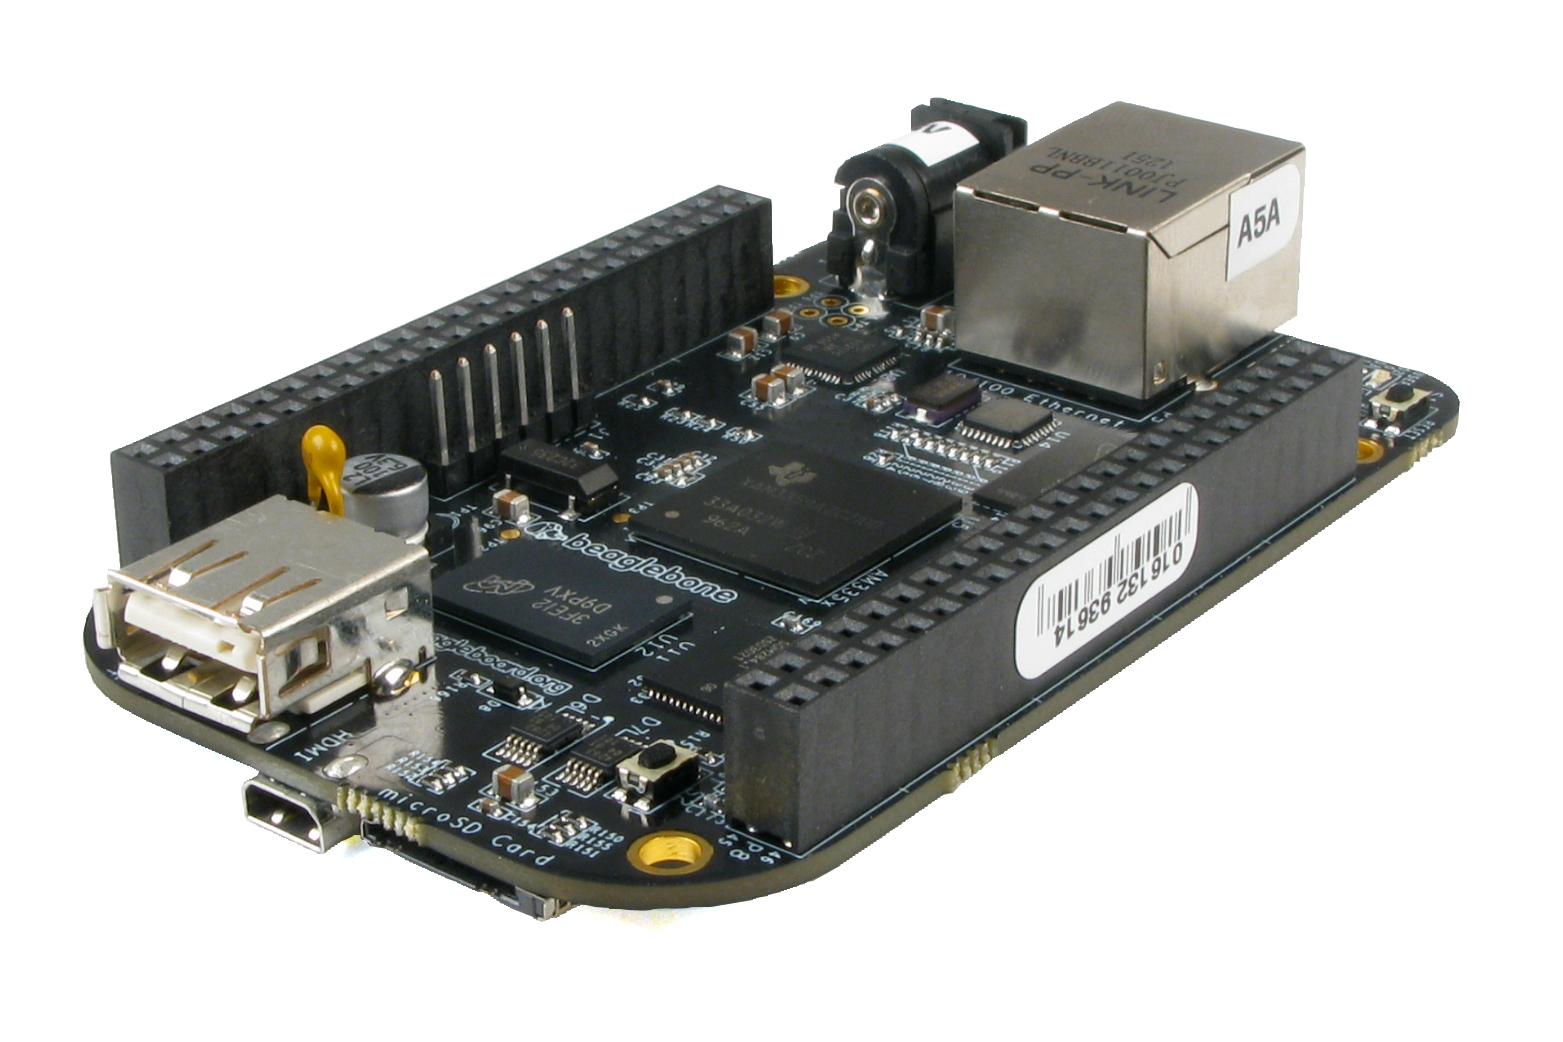
\includegraphics[scale=0.10]{./Resources/bbb.jpg}
 	\caption{Plataforma de Desenvolvimento - BeagleBone Black}
 	\label{bbb}
\end{figure}

A segunda plataforma a ser utilizada e estudada é a plataforma Jetson TK1 produzida pela NVIDIA, figura \ref{jetson_tk1}. Essa plataforma conta com um processador de 32-bits Tegra K1 baseado na tecnologia ARM Cortex-A15. O motivo pelo qual esta plataforma foi escolhida é devido ao seu poder de processamento gráfico, visto que apresenta 192 núcleos gráficos, sendo assim adequada para aplicações envolvendo processamento de imagens. A tabela \ref{jetson_tk1_tab} apresenta as especificações da plataforma.

\begin{table}[]
\centering
\caption{Especificações - Jetson TK1}
\label{jetson_tk1_tab}
\begin{tabular}{ll}
\textbf{Processador}           & NVIDIA 2.32GHz ARM quad-core Cortex-A15              \\
\textbf{Processador Gráfico}   & NVIDIA Kepler "GK20a" GPU  with 192 SM3.2 CUDA cores \\
\textbf{DRAM}                  & 2GB DDR3L 933MHz EMC x16 using 64-bit data width     \\
\textbf{Armanezamento}         & 16GB fast eMMC 4.51 (routed to SDMMC4)               \\
\textbf{Sistemas Operacionais} & Platforma 64-bit Linux Ubuntu 14.04                  \\
\textbf{Consumo de energia}    & 0.6W to 3W @ 12 V                                    \\
\textbf{Pinos de GPIO}         & 7 x GPIO pins (1.8V)                                 \\
\textbf{Periféricos}           & USB, mini-PCIe, SATA, SD-card, HDMI, audio          
\end{tabular}
\end{table}

\begin{figure}[H]
 	\centering
 	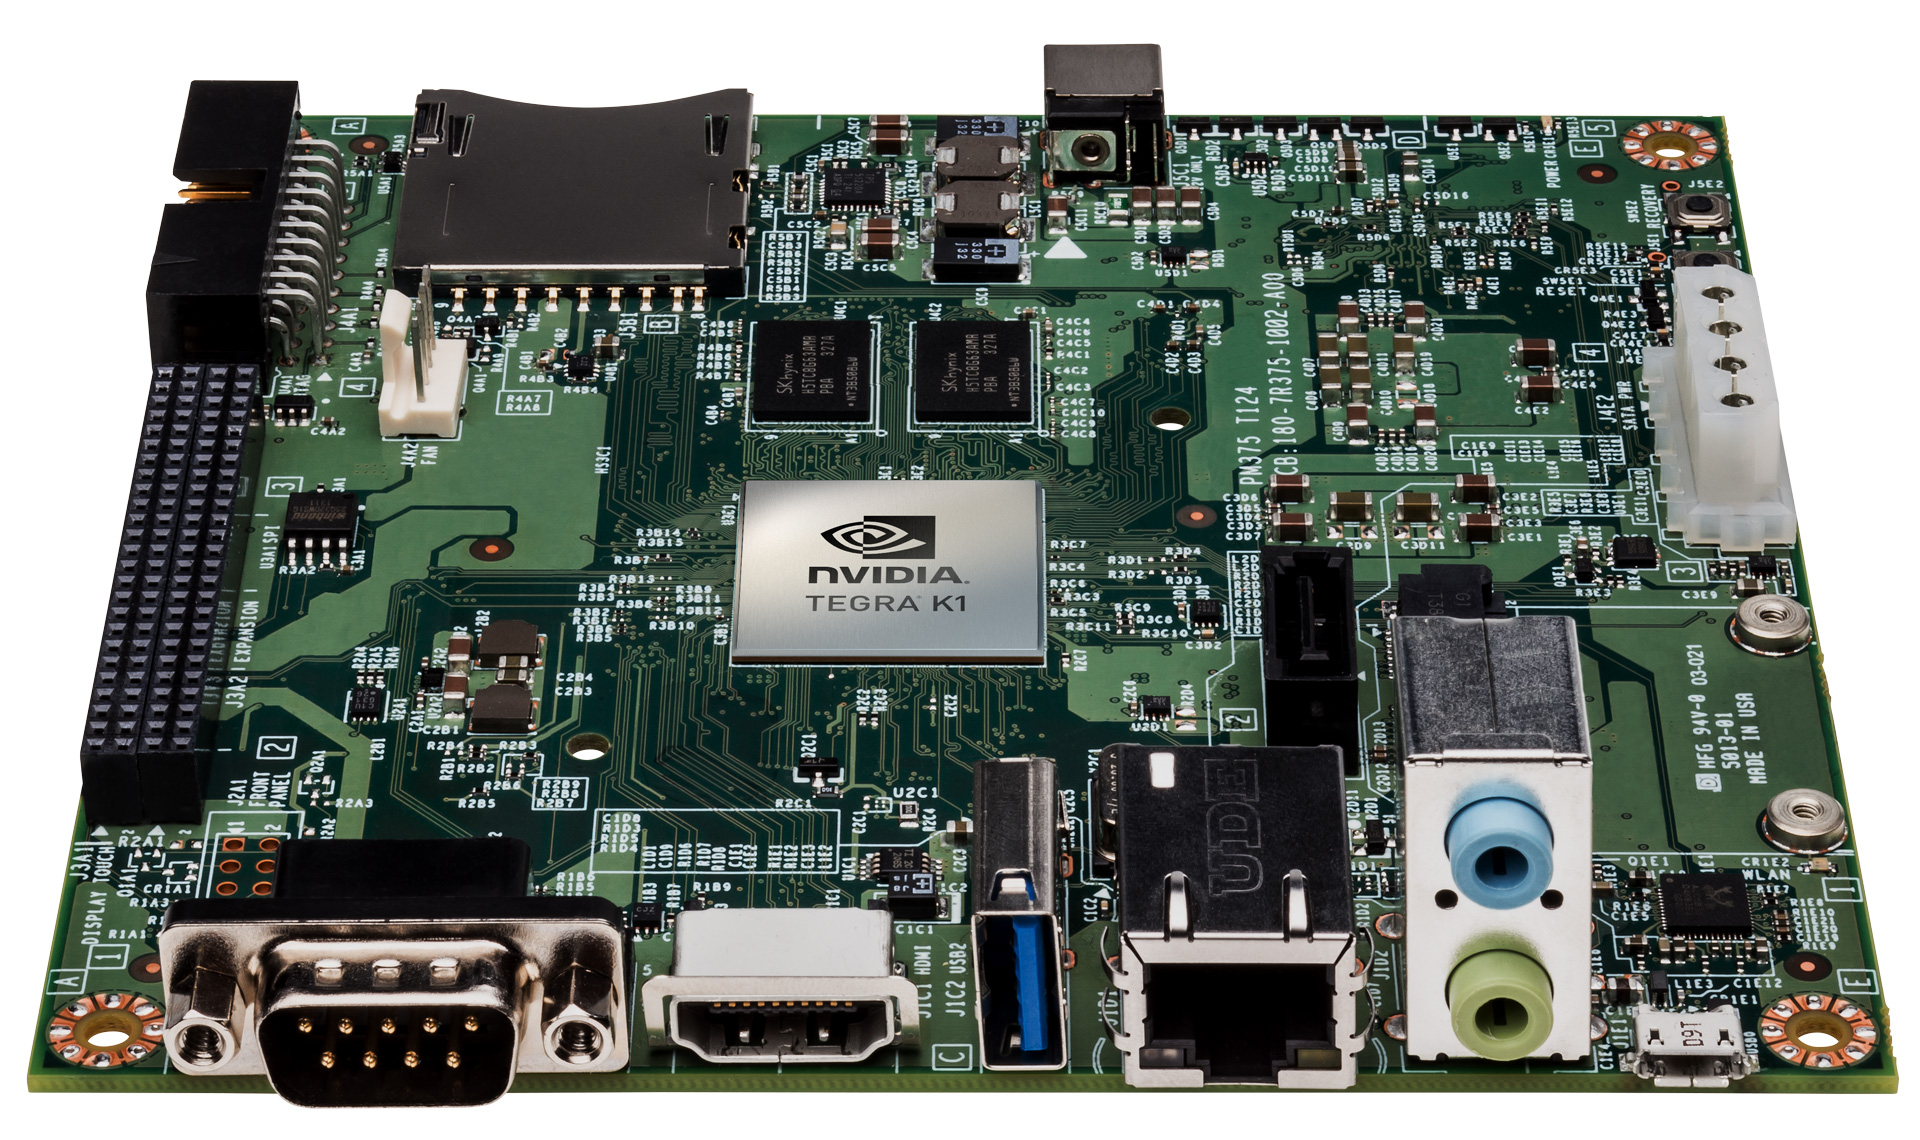
\includegraphics[scale=0.10]{./Resources/jetson_tk1.jpg}
 	\caption{Plataforma de Desenvolvimento - Jetson TK1}
 	\label{jetson_tk1}
\end{figure}

\subsection{Equipamentos auxiliares}

Abaixo estão apresentados os equipamentos auxiliares para o desenvolvimento do trabalho. 

Os métodos para a identificação de correspondências entre as câmeras requerem que a imagem estejam calibradas e retificadas. Por conta disso, utiliza-se o padrão de calibração de dimensão 7x10, apresentado na figura \ref{calibration_pattern}, para este propósito. Deste modo, é possível caracterizar as distorções das lentes, parâmetros intrínsecos, e o posicionamento de uma das câmeras com relação a outra, parâmetros extrínsecos.  

\begin{figure}[H]
 	\centering
 	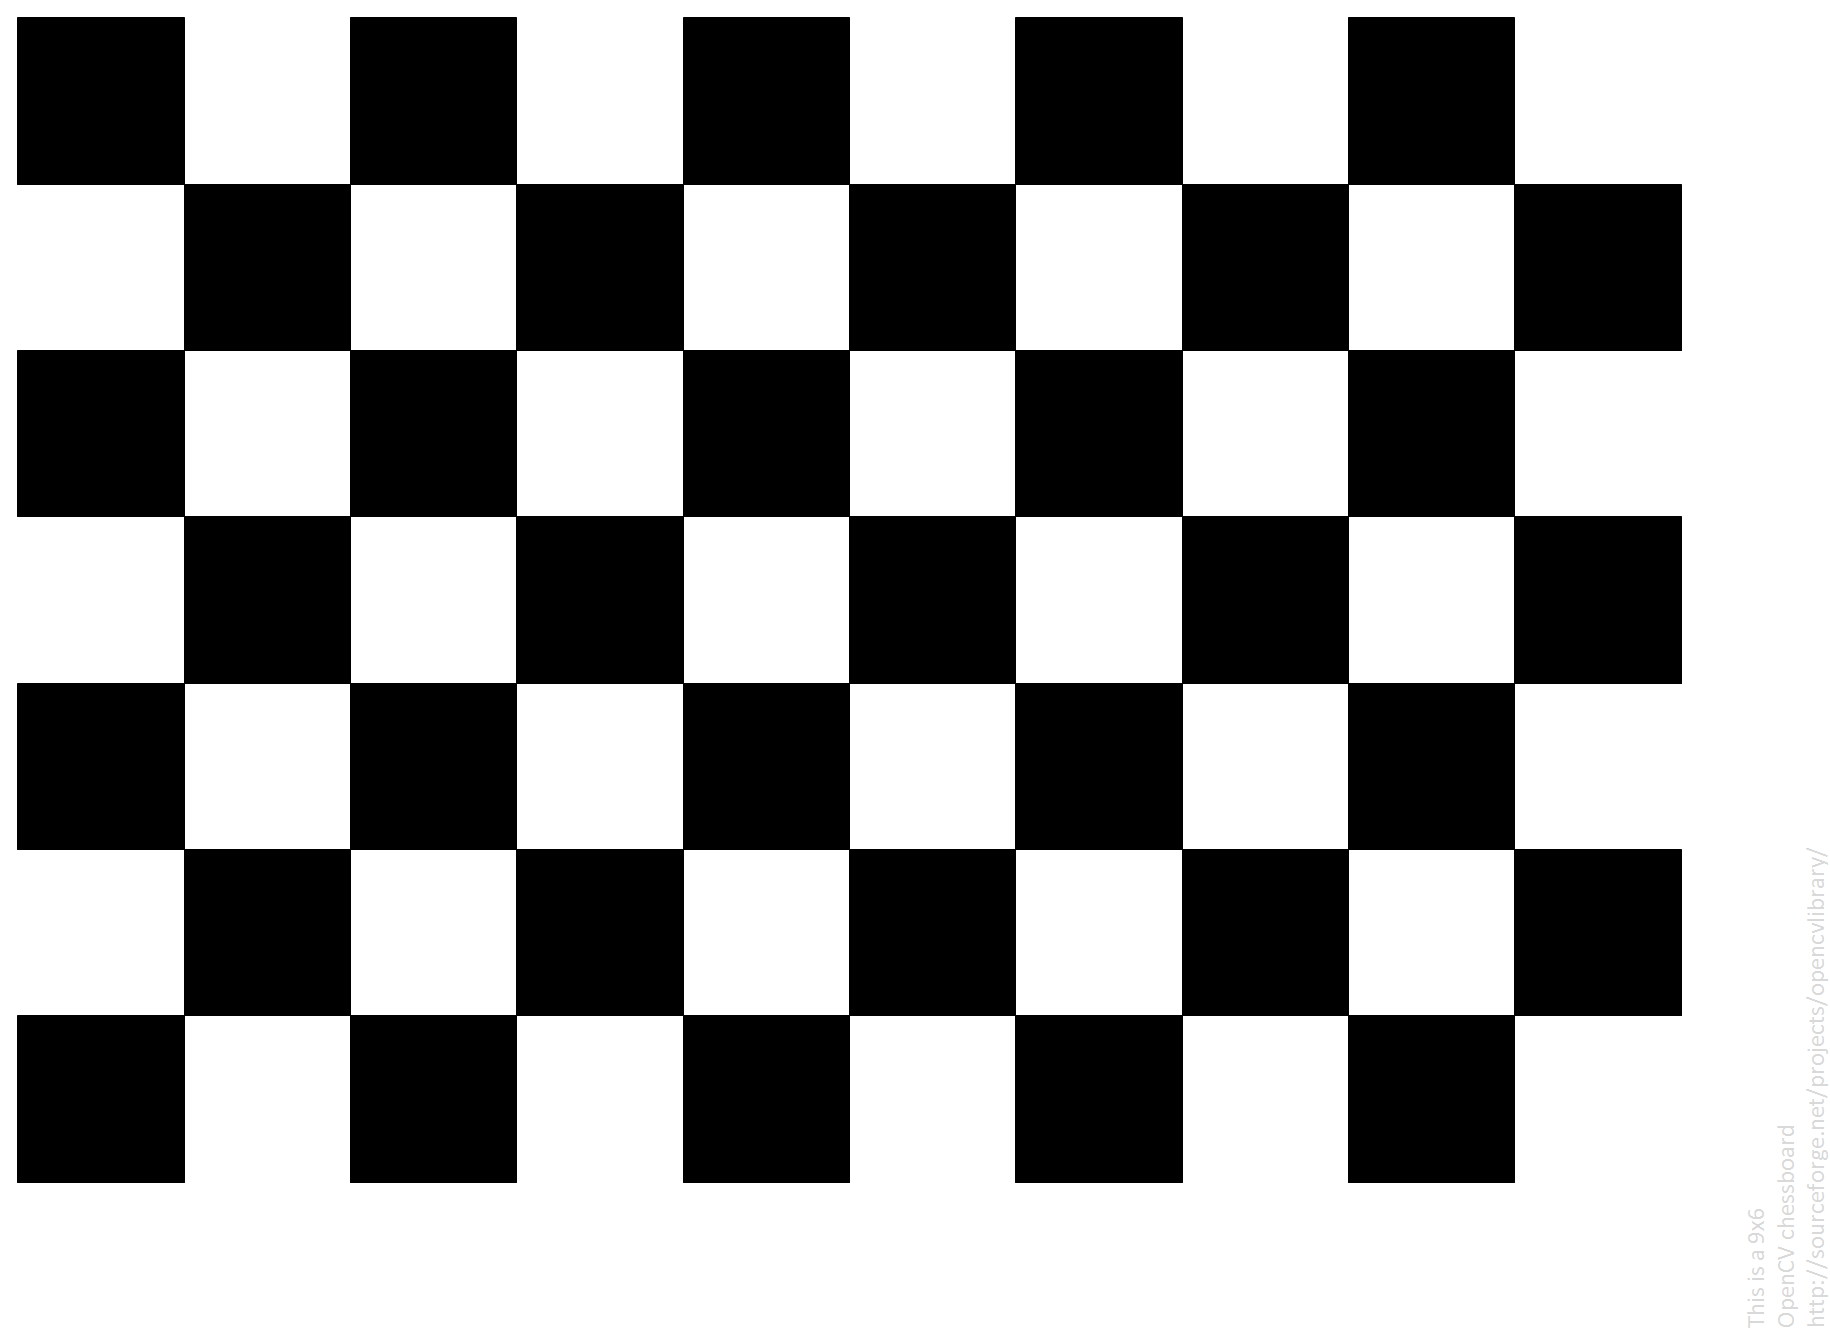
\includegraphics[scale=0.10]{./Resources/calibration_pattern.png}
 	\caption{Padrão de Calibração}
 	\label{calibration_pattern}
\end{figure}

A motivação deste trabalho é a sua utilização em veículos aéreos. Por conta disso, é indispensável que se tenha algum desses veículos. O trabalho conta com a utilização de um quadricóptero produzido pela 3DR, porém este apresenta modificações visando o seu desenvolvimento para navegação autônoma. Deste modo, tem-se a adição de \textit{propellers guards}, objetivando o aumento da segurança do veículo e das pessoas que o operam. Além disso, o \textit{drone} conta com suportes para a câmera estereoscópica e para a plataforma embarcada. Como pode ser observado pela figura \ref{quad_camera_support}, todas as peças foram produzidas utilizando impressora 3D.

\begin{figure}[H]
 	\centering
 	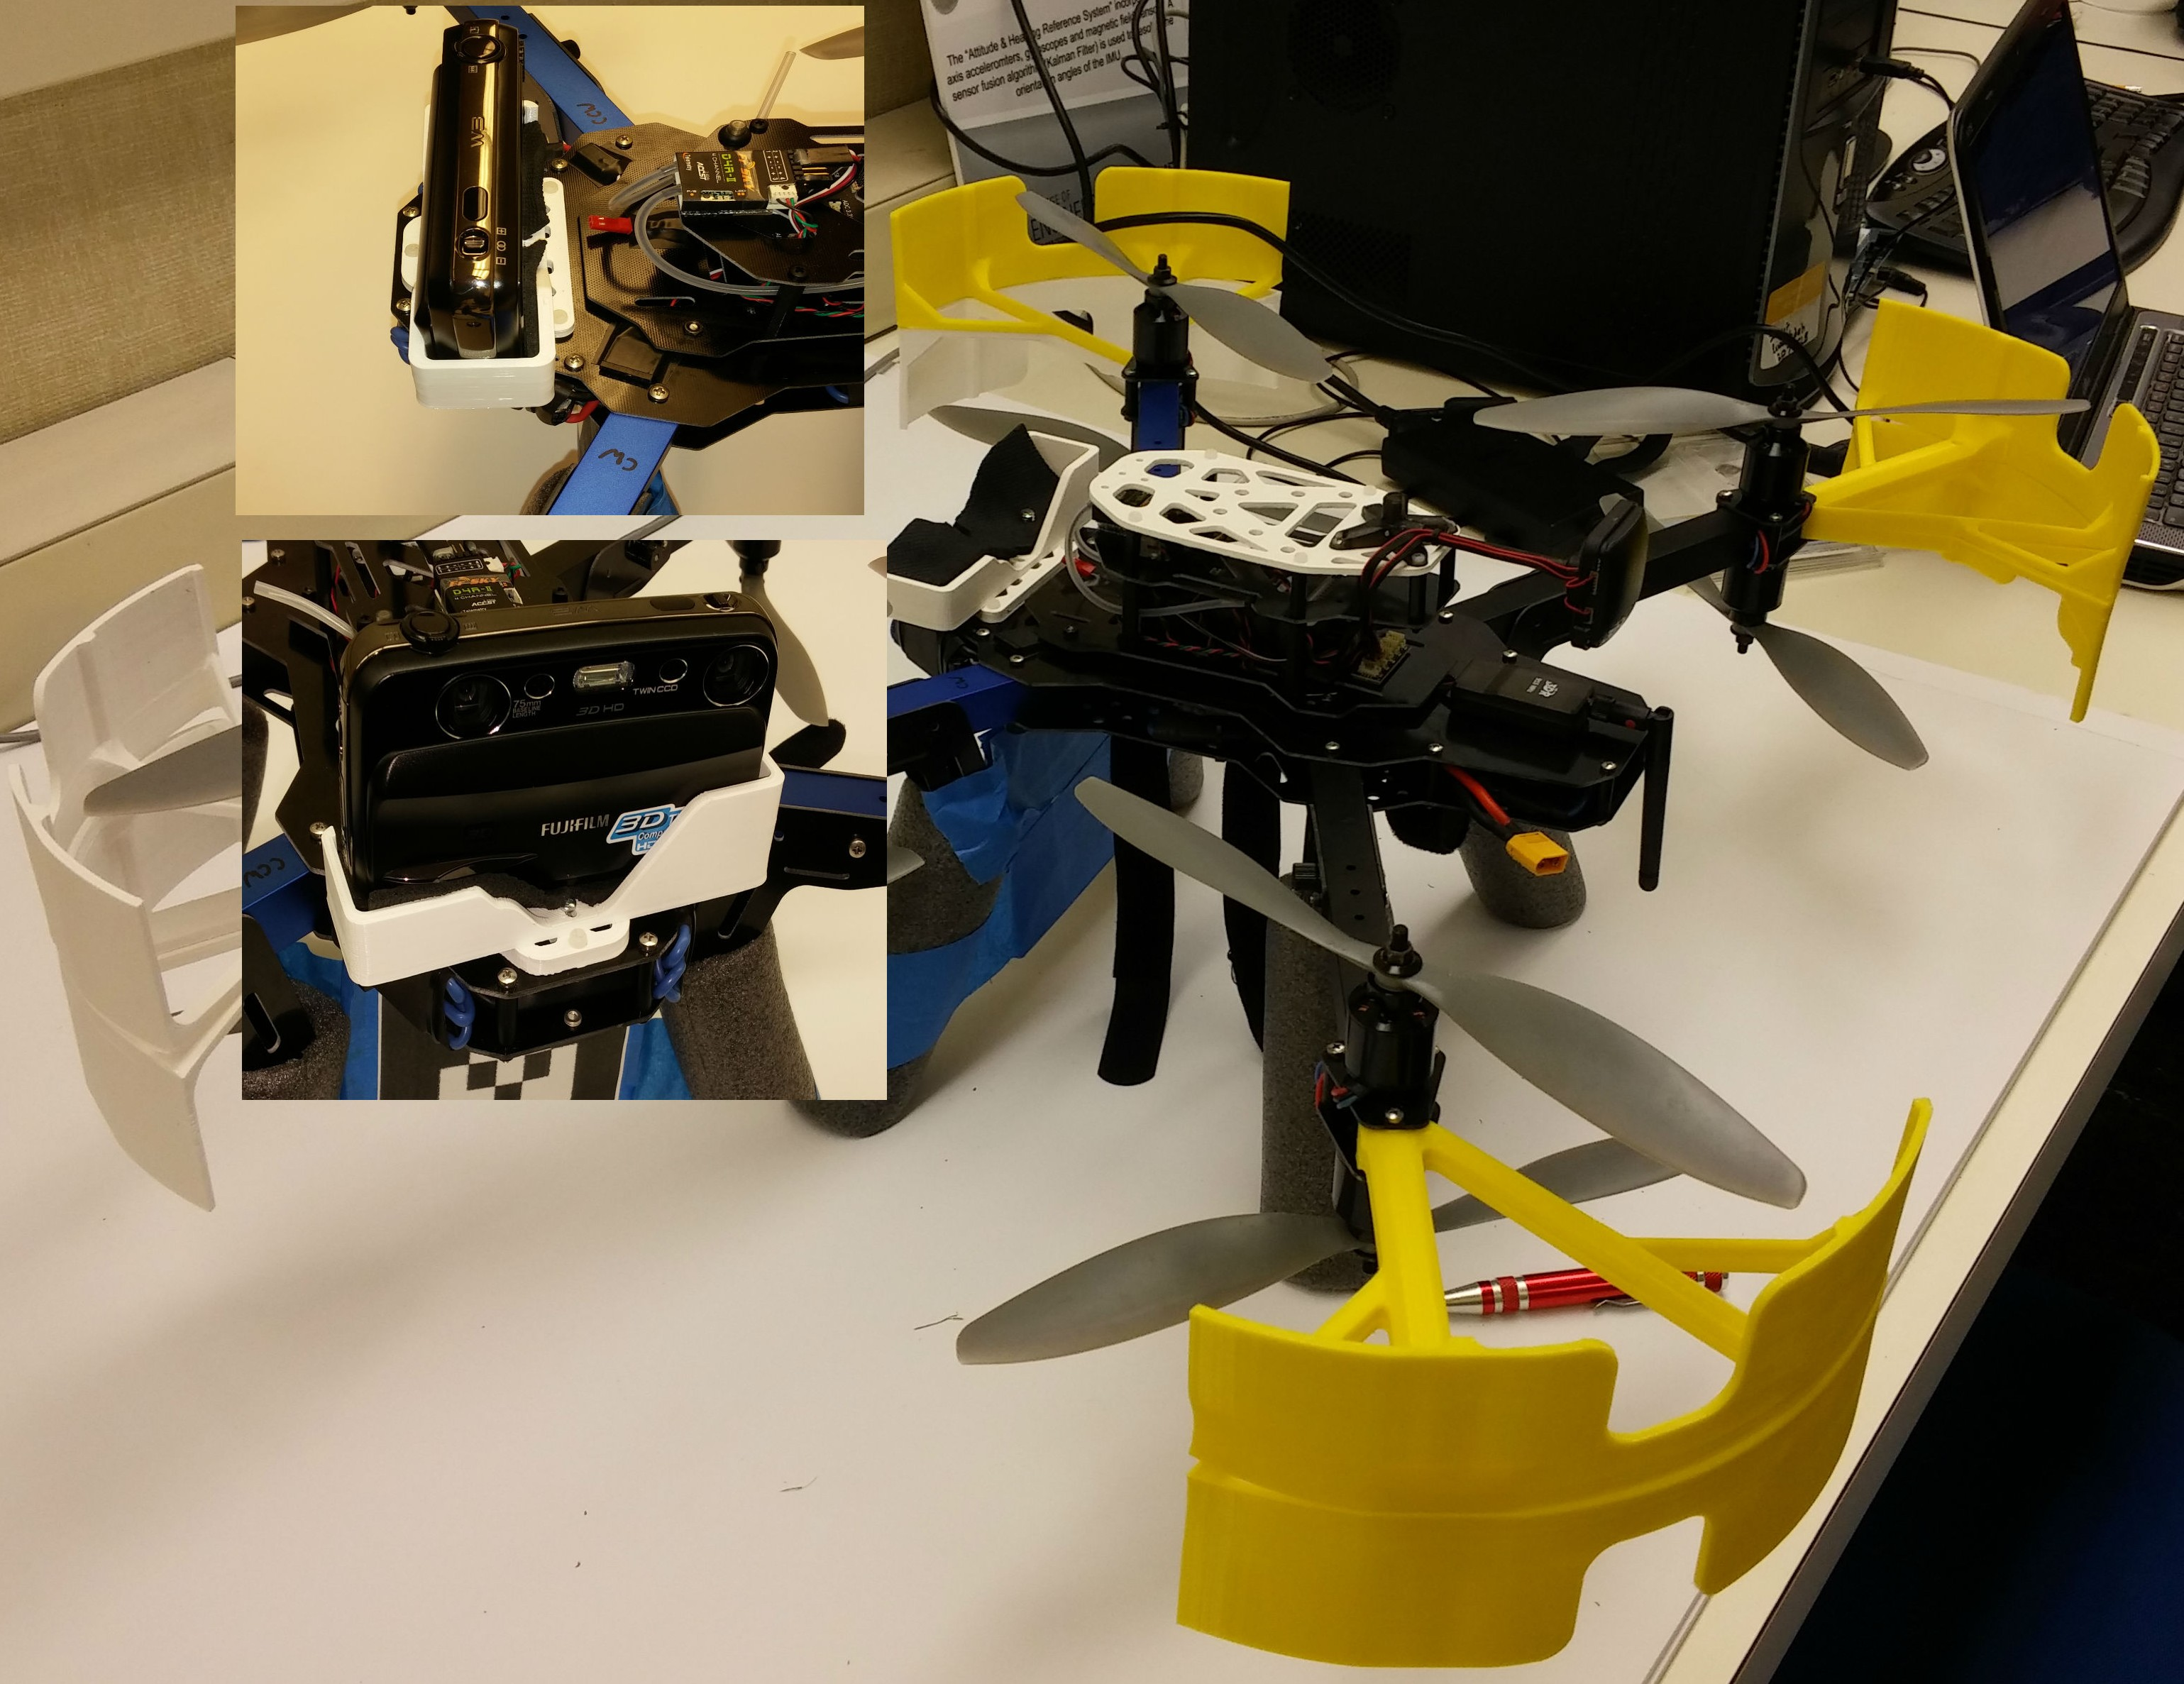
\includegraphics[scale=0.10]{./Resources/quad_camera_support.jpg}
 	\caption{Quadricóptero 3DR X8 com suporte para a Câmera 3D}
 	\label{quad_camera_support}
\end{figure}

%------------------------------------ Métodos -------------------------------------------------------
\section{Métodos}

Nesta seção serão apresentados os cenários e os métodos utilizado para o desenvolvimento do algoritmo para a detecção de obstáculos.

\subsection{Cenários}

O algoritmo de detecção de obstáculos desenvolvido tenta contornar todas as adversidades propostas pelos seguintes cenários. Propôs-se que ele deve ser flexível à variações na luminosidade, capaz de detectar obstáculos estáticos e móveis, e ser imune à vibrações. Deste modo, dois cenários em ambiente confinado e um em ambiente aberto foram analisados. Deseja-se a navegação autônoma ocorra até mesmo em casos que o sinal do Sistema de Posicionamento Global (GPS) seja perdido, por conta disso escolheu-se a utilização dos ambientes confinados. O ambiente externo foi escolhido devido a quantidade de fatores que poderiam atrapalhar e tornar o algoritmo mais robusto.

\subsubsection{Cenário 1}

O cenário da figura \ref{thumb_video10_l} foi utilizado para estudo das condições de ambiente externo, o qual está sujeito grandes variações de luminosidade e um número menor de movimentos, o que permite uma análise de alcances maiores. O principal  obstáculo deste cenário é uma árvore. 

\begin{figure}[H]
 	\centering
 	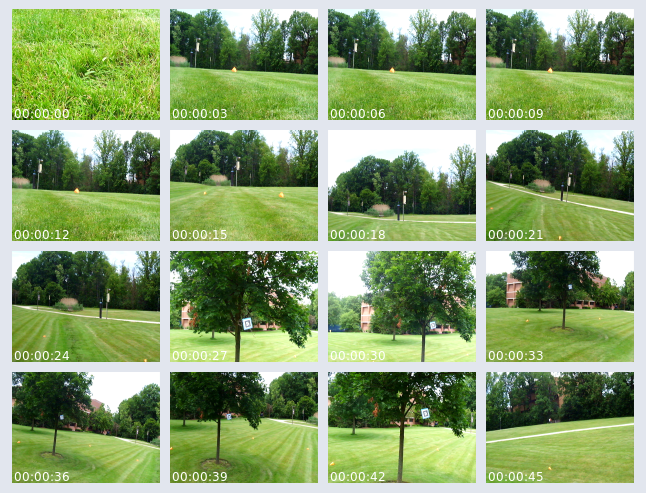
\includegraphics[scale=0.50]{./Resources/thumb_video10_l.png}
 	\caption{Cenário 1 - Ambiente Externo - Árvore}
 	\label{thumb_video10_l}
\end{figure}

\subsubsection{Cenário 2}

O cenário da figura \ref{thumb_video12_l} foi utilizado para estudo das condições de ambiente interno, o qual também apresenta certa variação de luminosidade, porém apresenta um número maior de movimentos, permitindo uma análise de objetos estáticos à curta e média distância. Os principais obstáculos deste cenário são uma mesa, uma cadeira e duas estantes.

\begin{figure}[H]
 	\centering
 	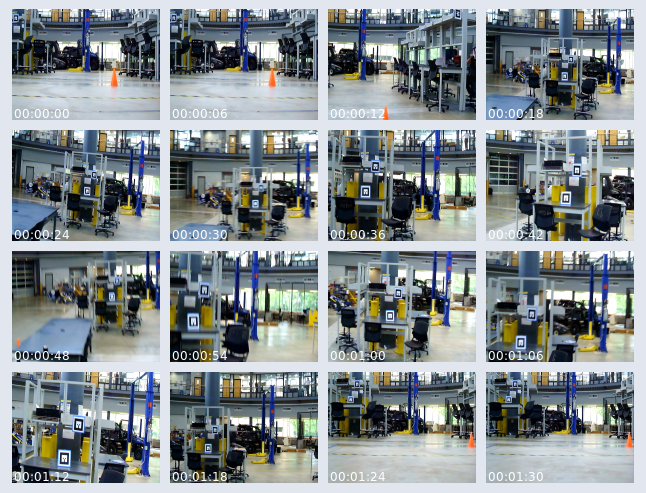
\includegraphics[scale=0.50]{./Resources/thumb_video12_l.png}
 	\caption{Cenário 2 - Ambiente Interno - Mesa/Cadeira/Estantes}
 	\label{thumb_video12_l}
\end{figure}

\subsubsection{Cenário 3}

O cenário da figura \ref{thumb_video15} foi utilizado para estudo das condições de ambiente interno, o qual também apresenta certa variação de luminosidade, apresenta um número muito maior de movimentos e permite a análise de objetos móveis à curto e médio alcance. Os principais obstáculos deste cenário  é uma bancada e um outro quadricóptero no campo de visão do veículo pilotado.

\begin{figure}[H]
 	\centering
 	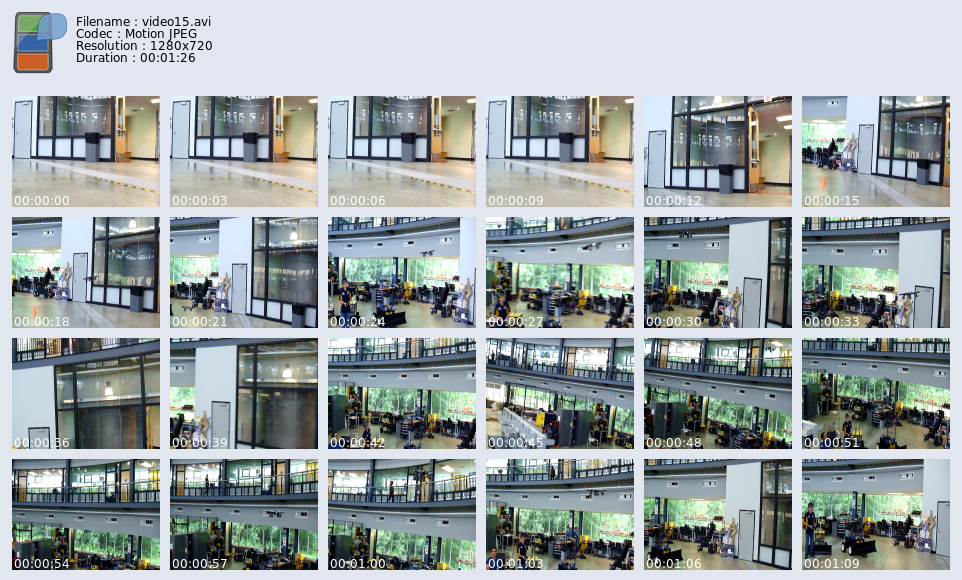
\includegraphics[scale=0.50]{./Resources/thumb_video15.png}
 	\caption{Cenário 3 - Bancada/Quadricóptero}
 	\label{thumb_video15}
\end{figure}


\subsection{Processamento de Imagem}

Nessa seção será apresentado o processamento de imagens utilizado para a identificação de obstáculos. Como pode ser visto na figura \ref{stereo_processor_steps}, todo o processo conta com seis etapas.

\textbf{Câmeras:} O primeiro passo do processo é a captura das imagens da câmera estereoscópica. Idealmente, as imagens deve ser capturadas ao mesmo instante e as lentes não apresentarem distorções.   

\textbf{Calibração e Retificação:} Na prática, as lentes apresentam distorção. Com base nos parâmetros obtidos após a calibração das câmeras é possível retificá-las. 

\textbf{Correspondência Estéreo:} Aplica-se os métodos para encontrar as correspondências entre as duas câmeras, gerando assim o mapa de disparidades.

\textbf{Pré-filtragem:} Este passo, pode ser aplicado tanto nas imagens retificados ou no mapa de disparidades. Atualmente, aplica-se a operação morfológica de abertura e um filtro de Mediana sobre o mapa de disparidades. 

\textbf{Limiarização por Distância:} Visto que a disparidade apresenta uma relação com a distância, aplica-se uma operação de limiarização. Deste modo, apenas os obstáculos a uma certa distância são segmentados.

\textbf{Identificação de Obstáculos:} Após o passo anterior, o objeto é identificado e sua posição é rastreada. Essa informação pode ser utilizada pelo sistema de controle da aeronave para manter distância do obstáculo identificado.

\begin{figure}[H]
 	\centering
 	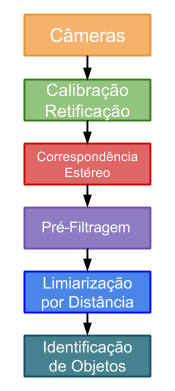
\includegraphics[scale=0.50]{./Resources/stereo_processor_steps.png}
 	\caption{Etapas do Processamento de Imagens}
 	\label{stereo_processor_steps}
\end{figure}

%\subsection{Métodos Estéreo }
%
%\subsubsection{Método Estéreo Local - \textit{Block Matching}}
%
%\subsubsection{Método Estéreo Semi-global - \textit{Semi-global Block Matching}}
